\documentclass[final]{beamer}

% ====================
% Packages
% ====================

\usepackage[T1]{fontenc}
\usepackage{lmodern}
\usepackage[size=a0,scale=1.0]{beamerposter}
\usetheme{gemini}
\usecolortheme{ITNU}
\usepackage{graphicx}
\usepackage{booktabs}
\usepackage{svg}
\usepackage{pgfplots}
\usepackage{caption}
\usepackage{subcaption}

% for circling parts
\usepackage{graphicx}
\usepackage[usestackEOL]{stackengine}
\usepackage{xcolor}
\def\calloutsym{%
  \ensurestackMath{%
  \scalebox{3.5}{\color{red}\stackunder[0pt]{\bigcirc}{\downarrow}}}%
}
\newcommand\callouttext[1]{%
  \def\stacktype{S}\renewcommand\useanchorwidth{T}\stackText%
  \stackunder{\calloutsym}{\scriptsize\Longstack{#1}}\stackMath%
}
\newcommand\callout[3][1.5pt]{%
  \def\stacktype{L}\stackMath\stackunder[#1]{#2}{\callouttext{#3}}%
}

% ====================
% Lengths
% ====================

% If you have N columns, choose \sepwidth and \colwidth such that
% (N+1)*\sepwidth + N*\colwidth = \paperwidth
\newlength{\sepwidth}
\newlength{\colwidth}
\setlength{\sepwidth}{0.001\paperwidth}
\setlength{\colwidth}{0.3\paperwidth}

\newcommand{\separatorcolumn}{\begin{column}{\sepwidth}\end{column}}

% ====================
% Title
% ====================

\title{CS6216 Project Report: Stein Variational Gradient Descent}

\author{Apivich Hemachandra\inst{1} \and
Jiashu Tao\inst{1} \and
Bo Wang\inst{1}   \and
Jiayuan Ye\inst{1} }
\institute{Department of Computer Science,  National University of Singapore\\{\small\textsuperscript{*}Alphabetical Order.}}

% remove this section if poster is for inhouse project
\addtobeamertemplate{headline}{} 
{
    \begin{tikzpicture}[remember picture,overlay]
    % tweak these sizes according to the logo of the company:
    % xshift, yshift, height
    \node [anchor=north west, inner sep=3cm] at ([xshift=-1.5cm,yshift=-0.8cm]current page.north west)     {
\includegraphics[height=3cm]{imgs/logo.png}}; 
    \end{tikzpicture} 
}

% ====================
% Body
% ====================

\begin{document}

\begin{frame}[t]
\begin{columns}[t]

\separatorcolumn

\begin{column}{\colwidth}

\begin{block}{Problem Setting}

\begin{itemize}
    \item The aim is to generate a set of particles that provides a good approximation of some probability distribution. This is useful in Bayesian inference problem.
    
    \item The work uses Stein discrepancy to develop a variational inference method that works for a general inference problem and is also scalable.
\end{itemize}

\begin{center}
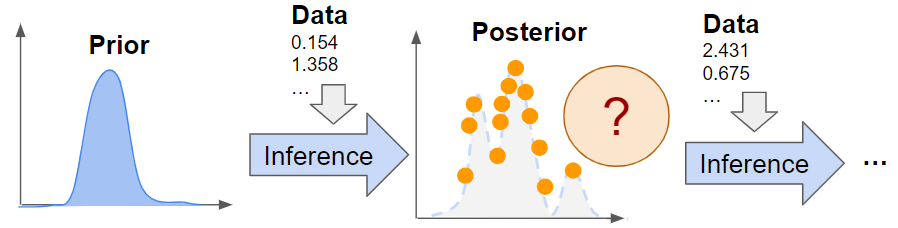
\includegraphics[width=0.6\textwidth]{figs/setting.png}
\end{center}

\end{block}

\begin{block}{SVGD Algorithm}

\textbf{Bayesian Inference via Variational Gradient Descent~\cite{liu2016stein}}

\begin{itemize}
    \item {\bfseries Input:} A target distribution with density function $p(x)$ and a set of initial particles $\{x_i^0\}_{i=1}^n$.
    \item {\bfseries Output:} A set of particles $\{x_i\}_{i=1}^n$ that approximates the target distribution.
    \item {\bfseries Iterative Particle update:} for iteration $\ell$, $x_i^{\ell+1}\leftarrow x_i^l + \epsilon_l \hat{\mathbf{\phi}}^*(x_i^\ell)$, 
	where $\hat{\mathbf{\phi}}^*(x) = \frac{1}{n} \sum_{j=1}^n\left[ k(x_{j}^\ell, x)\nabla_{x_j^\ell}\log p(x_j^\ell) + \nabla_{x_j^\ell} k(x_j^\ell, x)\right]$
\end{itemize}
\end{block}

  \begin{block}{Experiment: Toy Example of One-dimensional Gaussian Mixture}
    
\newcommand{\toyfigwidth}{0.9\textwidth}
\begin{figure}[!htbp]
    \centering
    % \begin{tabular}{@{}c@{}}
    %     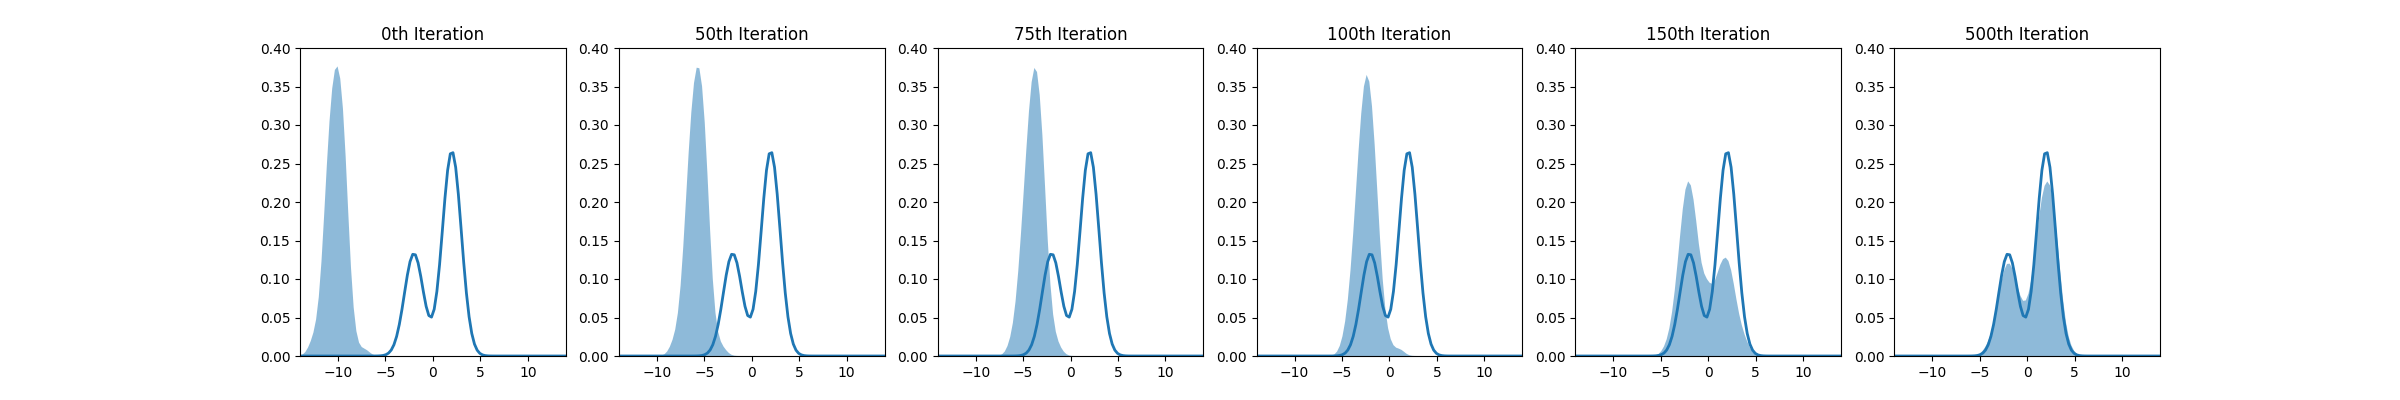
\includegraphics[width=\toyfigwidth]{figs/toy-figure1_step0.1_mu2.0_w0.33_gaussian.png} \\
    %     \small (1) StepSize = 0.1, 500 iterations, $\mu = \pm 2$, $(w_1, w_2) = (0.33, 0.67)$
    % \end{tabular}
    
    \begin{tabular}{@{}c@{}}
        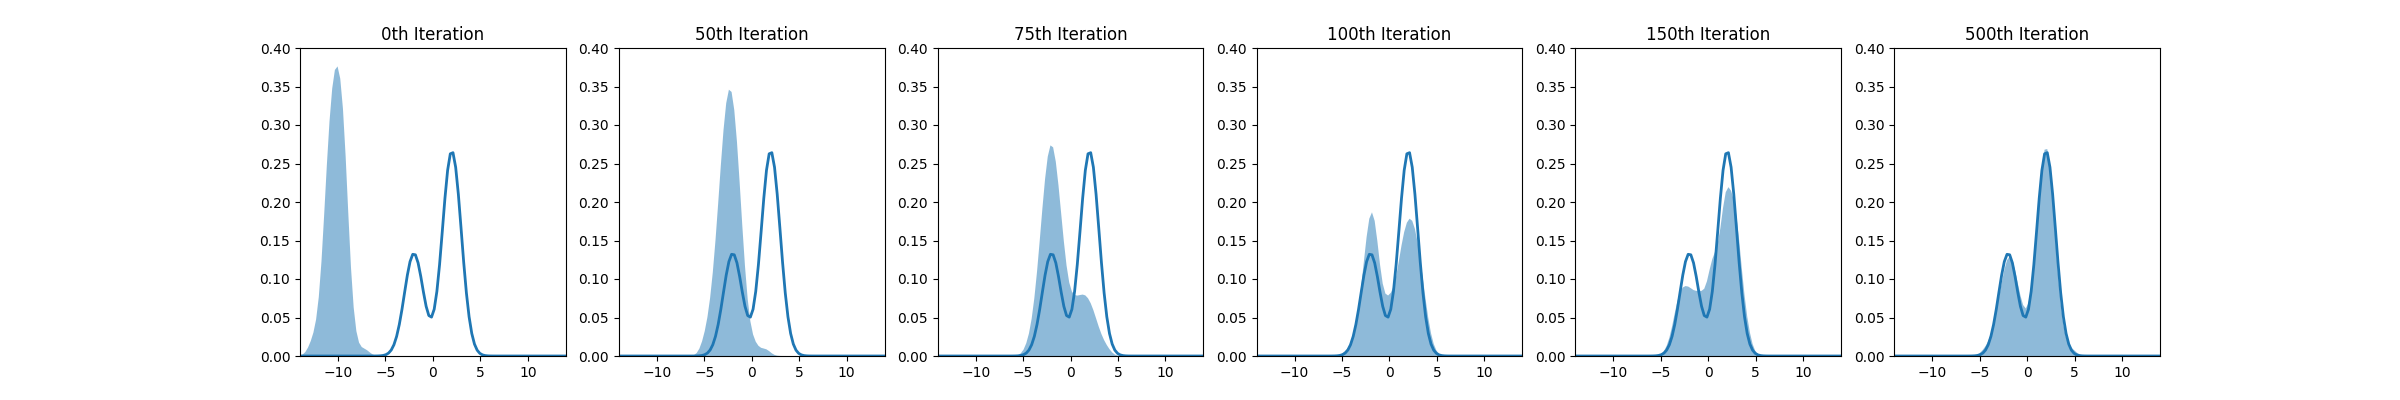
\includegraphics[width=\toyfigwidth]{figs/toy-figure1.png} \\
        \small (1) StepSize = 0.25, 500 iterations, $\mu = \pm 2$, $(w_1, w_2) = (0.33, 0.67)$
    \end{tabular}
    %\vspace{\floatsep}
    
    \begin{tabular}{@{}c@{}}
        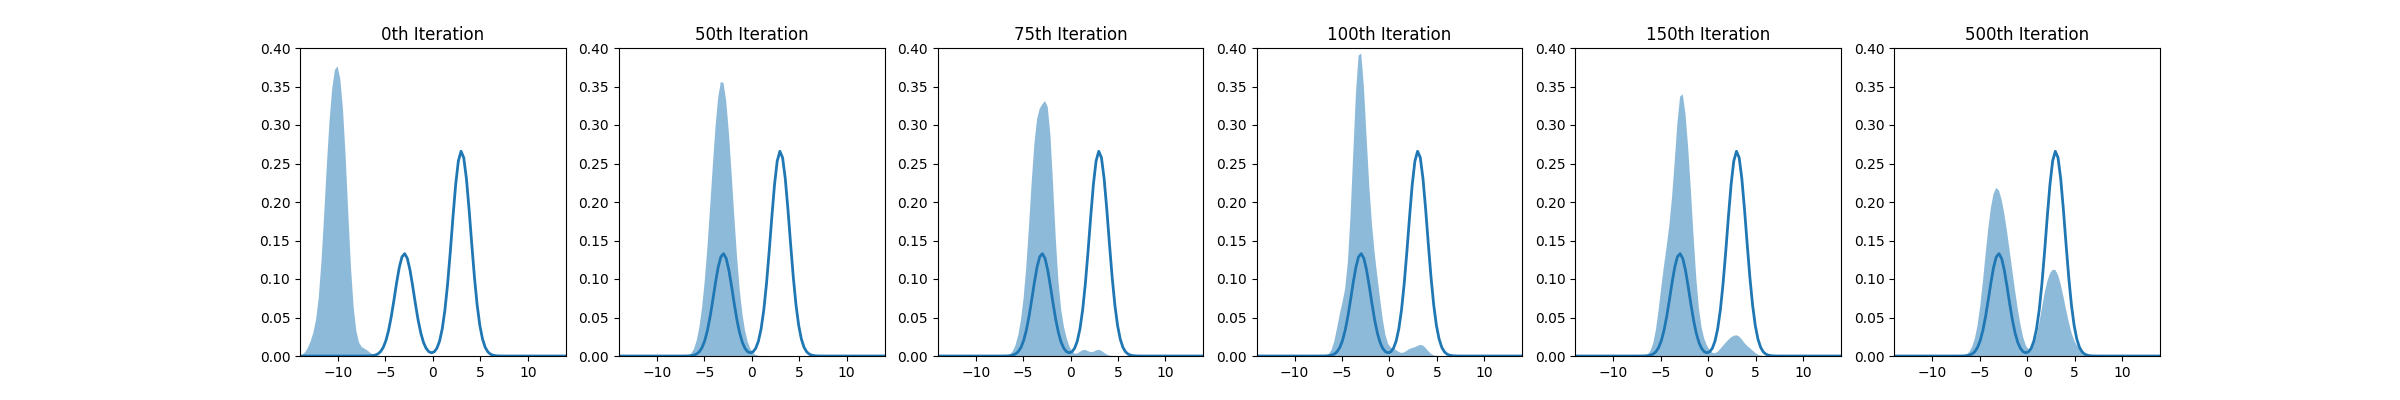
\includegraphics[width=\toyfigwidth]{figs/toy-figure1_step0.25_mu3.0_w0.33_gaussian.png} \\
        \small (2) StepSize = 0.25, 500 iterations, $\mu = \pm 3$, $(w_1, w_2) = (0.33, 0.67)$
    \end{tabular}
    
    \begin{tabular}{@{}c@{}}
        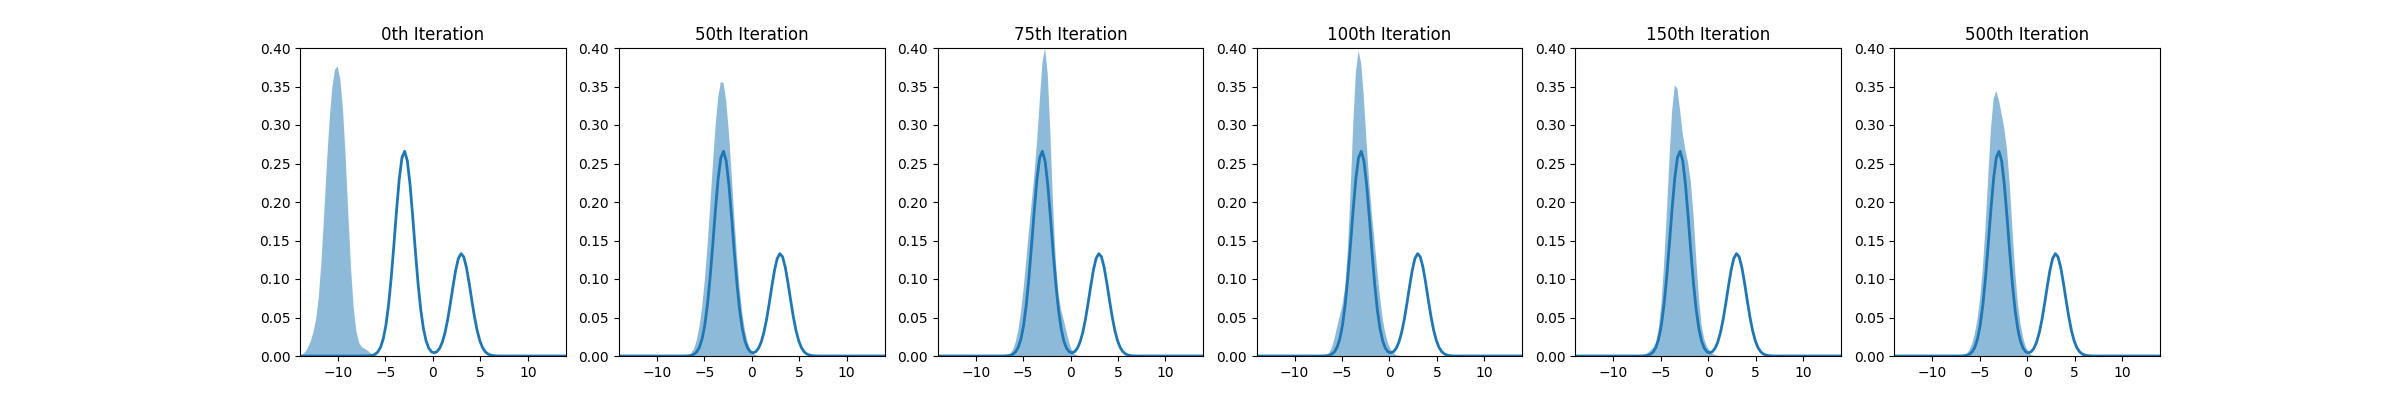
\includegraphics[width=\toyfigwidth]{figs/toy-figure1_step0.25_mu3.0_w0.67_gaussian.png} \\
        \small (3) StepSize = 0.25, 500 iterations, $\mu = \pm 3$, $(w_1, w_2) = (0.67, 0.33)$
    \end{tabular}
    
    % \begin{tabular}{@{}c@{}}
    %     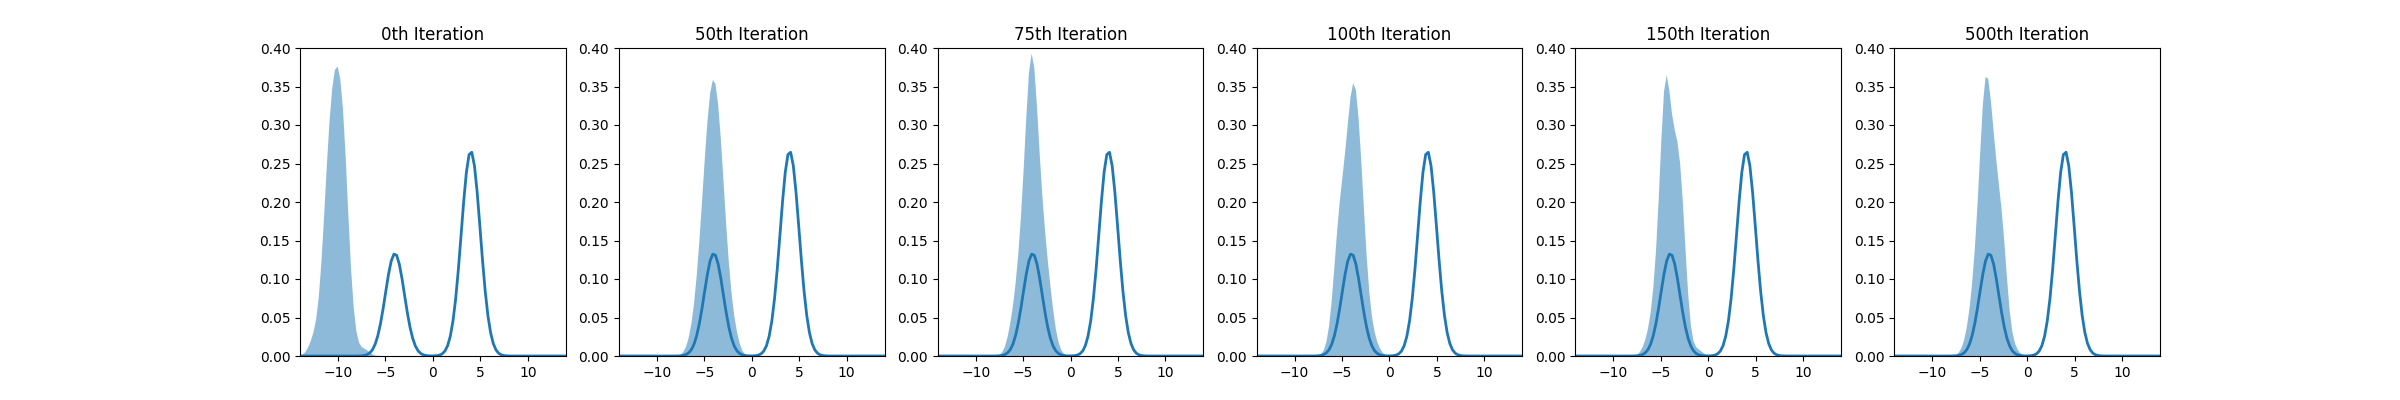
\includegraphics[width=\textwidth]{figs/toy-figure1_step0.25_mu4.0_w0.33_gaussian.png} \\
    %     \small (5) StepSize = 0.25, $\mu = \pm 4$, $(w_1, w_2) = (0.33, 0.67)$
    % \end{tabular}
    
    \begin{tabular}{@{}c@{}}
        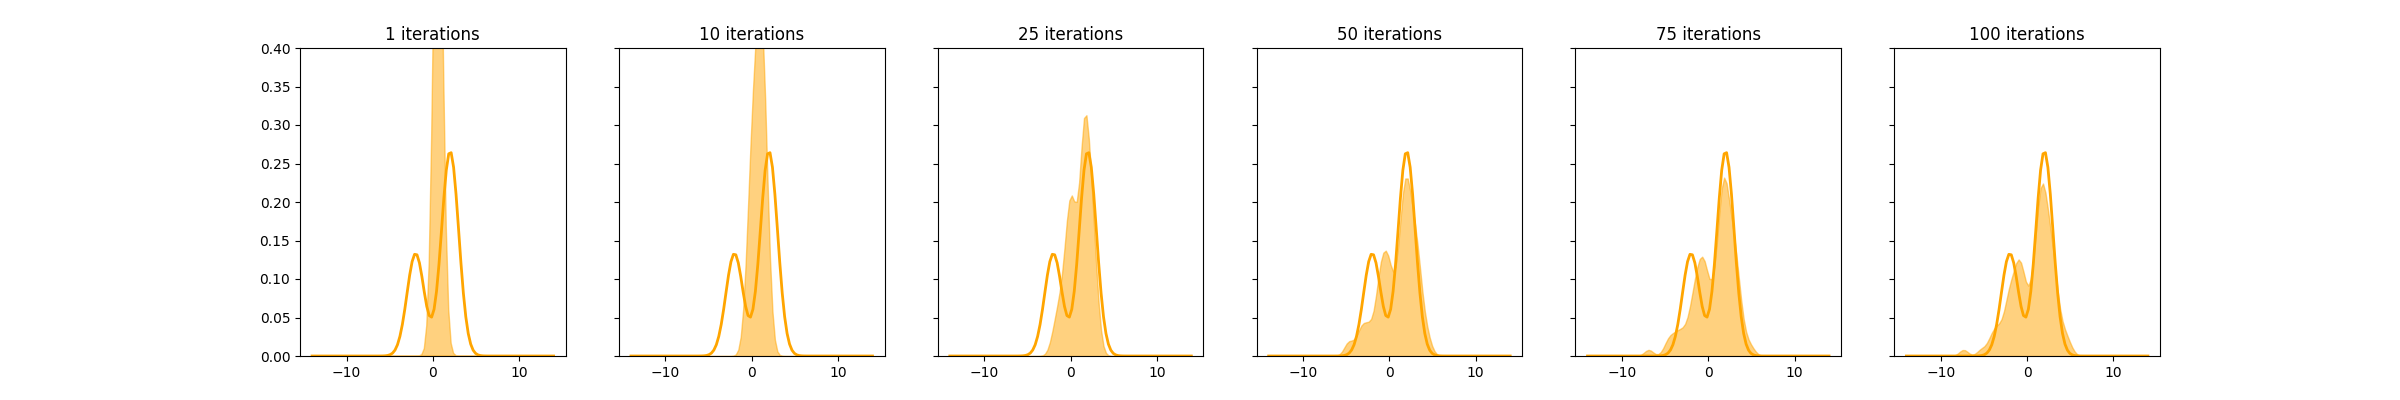
\includegraphics[width=\toyfigwidth]{figs/toy-figure1-numpyro.png} \\
        \small (4) ELBO Loss (NumPyro) StepSize = 0.1, 100 iters, $\mu = \pm 3$, $(w_1, w_2) = (0.33, 0.67)$
    \end{tabular}
     
    \caption{Toy example with 1D Gaussian mixture. Particle densities are visualized by KDE.}
    \label{fig:toy1dgaussian}
\end{figure}

    
    \begin{enumerate}
        \item When the two modes are far apart from each other, the SVGD algorithm converges more slowly, as in Figure 1. (2).
        \item When the smaller mode is far away from the initialization distribution, the particles in the SVGD algorithm have difficulty visiting the smaller mode, as in Figure 1. (3).
        \item Replacing the weighted negative log-likelihood $\rightarrow$ a single loss function such as the ELBO: This ELBO-within-Stein algorithm is implemented NumPyro, and we found that when applying it to Gaussian mixture, the particles seem to converge faster and only need 100 iterations, as in Figure 1. (4). 
    \end{enumerate}
  \end{block}
  


\end{column}

\separatorcolumn

\begin{column}{\colwidth}

% \textbf{Convergence of SVGD after finite number of iteration}
    


\begin{block}{Experiment: SVGD vs Monte Carlo for Mean Estimation}
    \begin{enumerate}
    \item SVGD performs better than Monte Carlo sampling (Smaller MSE).
    \item A larger step size for SVGD might converge faster but might also lead to a larger error.
    \end{enumerate}
    \begin{figure}[!htbp]
    \centering
    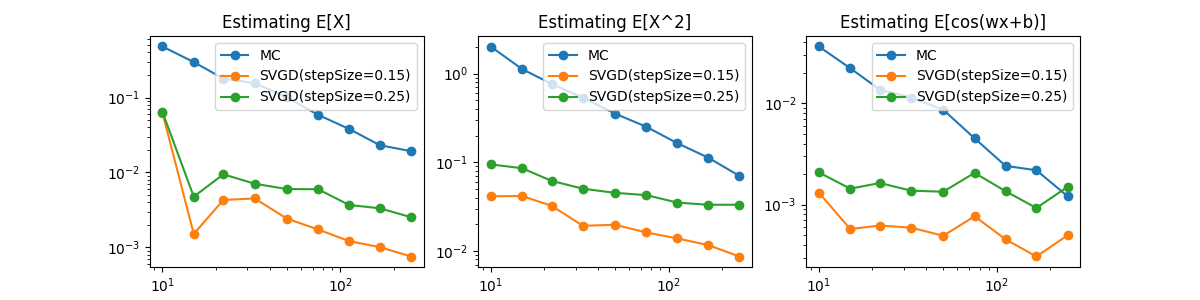
\includegraphics[width=\textwidth]{figs/toy-figure2-merged.png}
    \caption{Comparison between MC and SVGD on simple mean estimation tasks. }
    \label{fig:my_label}
\end{figure}

\end{block}

  \begin{block}{Experiment: Running Time vs \#Particles}

    \begin{itemize}
     \item \textbf{Tested Implementations:} SVGD (Original paper), NumPyro SteinVI (ELBO Loss)
     \item \textbf{Task:} Matching a multivariate Gaussian  \quad \textbf{Number of Particles:} 100\sim 1600
     \item \textbf{Machine:} AMD 3970X 32-Core CPU, 64GB RAM, GeForce RTX 3090 GPU.
    \end{itemize}
     \begin{figure}[!htbp]
    \centering
    \begin{tabular}{@{}cc@{}}
            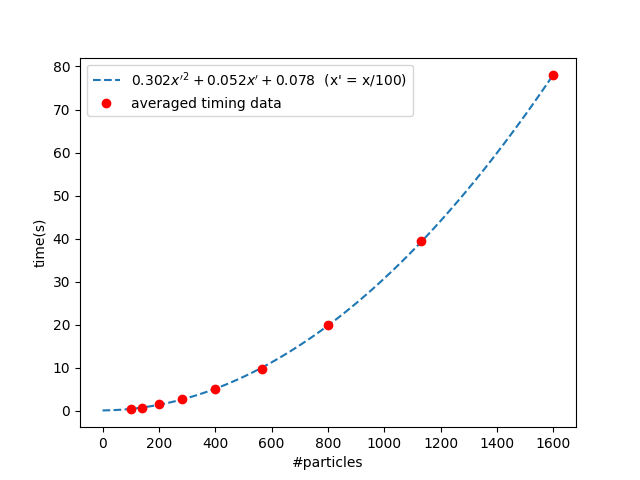
\includegraphics[width=0.40\textwidth]{figs/toy-timing-particles.png} & 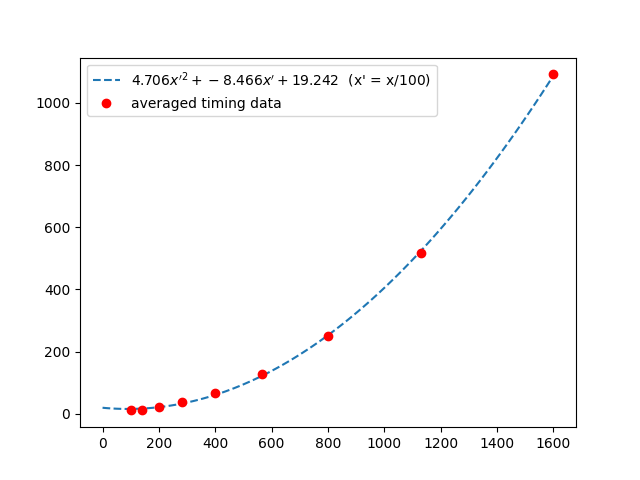
\includegraphics[width=0.40\textwidth]{figs/toy-timing-particles-numpyro-elbo.png}\\
        \small Original SVGD & NumPyro (ELBO Loss) \\
    \end{tabular}
    \caption{Timing vs particles }
    \label{fig:timingparticles}
\end{figure}

  \end{block}

\begin{block}{Experiment: Bayesian Logistic Regression on Small Datasets}
  \textbf{Logistic Regression:} On small datasets ($N \leq 10^4$)
    \begin{itemize}
     \item Compare the SVGD algorithm against the No U-Turn Sampler (NUTS) 
     
     \item Comparison using the accuracy of prediction and log-likelihood of test data
    \end{itemize}
     \begin{figure}[h]
    \centering
    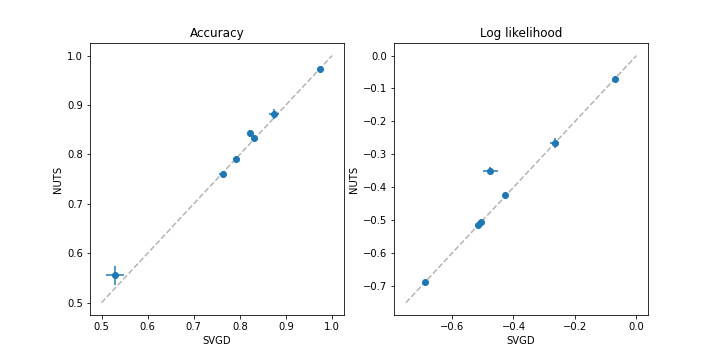
\includegraphics[width=0.6\textwidth]{figs/logistic_svgd_nuts.png}
    \caption{Comparison of accuracy (left) and log-likelihood (right) obtained by NUTS and SVGD algorithm on small-scale logistic regression dataset. The dotted line represents the situation where both algorithms perform as well was each other, and each point represent the average result on one of the dataset.}
    \label{fig:logist_small}
\end{figure}
  \end{block}

\end{column}

\separatorcolumn

\begin{column}{\colwidth}

  \begin{block}{Experiment: Bayesian Logistic Regression on Large Datasets}
  \textbf{Bayesian Linear Regression} on binary Covertype dataset 
    \begin{itemize}
     \item SVGD \cite{liu2016stein} consistently outperforms SGLD \cite{welling2011bayesian} in test accuracy
     \item SVGD is also more particle efficient than SGLD
     \item Training is noisier than what the paper reported originally
    \end{itemize}
    \begin{figure}[ht]
	\centering
	\begin{subfigure}[b]{0.45\textwidth}
		\centering
		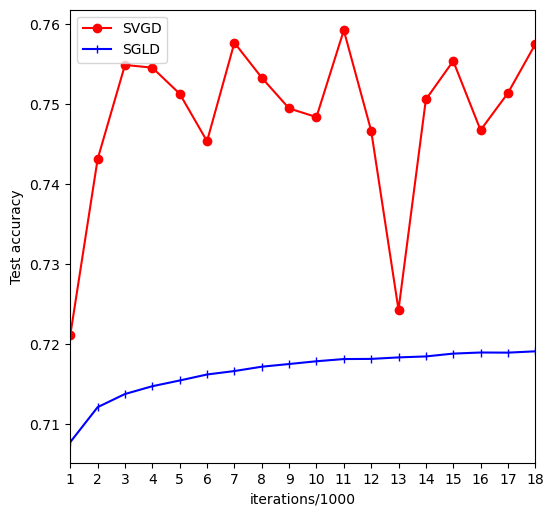
\includegraphics[height=0.2\textheight]{figs/sgvd_sgld_1.png}
		\caption{Test accuracy against every 1000 training iterations}
		\label{fig:acc_iter}
	\end{subfigure}
	\hfill
	\begin{subfigure}[b]{0.45\textwidth}
		\centering
		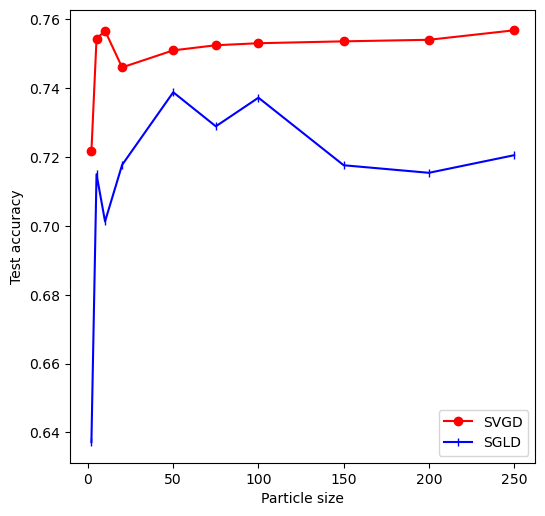
\includegraphics[height=0.2\textheight]{figs/sgvd_sgld_2.png}
		\caption{Test accuracy against number of particles at 3000 iterations ($\frac{1}{3}$ epochs)}
		\label{fig:acc_par}
	\end{subfigure}
	\caption{Results on Bayesian logistic regression on binary Covertype dataset for SVGD and SGLD. Left: Test accuracy against every 1000 training iterations. One epoch is roughly 9000 iterations given the batch size of 50. The number of particles used is 100. Right: Test accuracy against number of particles after 3000 training iterations are done. Experiments are done with 2, 5, 10, 20, 50, 75, 100, 150, 200, 250 particles. The dataset is divided into training and test set with a 8:2 ratio. Each experiment is done on 50 independent trials and the average number is reported.}
	\label{fig:covertype}
\end{figure}
  \end{block}
  
  \begin{block}{Experiment: Bayesian Neural Network}
  \begin{itemize}
      \item Compare the RMSE and log-likelihood between SVGD implementations and the probabilistic back-propagation (PBP) algorithm
      
      \item We are able to show that the original implementation of SVGD algorithm outperforms PBP, however, the NumPyro implementation often cannot perform as well
  \end{itemize}
  \begin{table}[]
    \centering
    \resizebox{\textwidth}{!}{
    \begin{tabular}{|c|ccc|ccc|}
    \hline
     & \multicolumn{3}{|c|}{Average RMSE} & \multicolumn{3}{|c|}{Average log-likelihood} \\
     \hline
    Dataset & PBP & SVGD (original) & SVGD (NumPyro) & PBP & SVGD (original) & SVGD (NumPyro) \\
        \hline
    Boston & $3.007 \pm 0.278$ & $2.987 \pm 0.341$ & $3.290 \pm 0.369$ & $-2.879 \pm 0.261$ & $-2.689 \pm 0.158$ & $-2.809 \pm 0.043$ \\
    Concrete & $5.435 \pm 0.075$ & $5.240 \pm 0.134$ & $5.567 \pm 0.158$ & $-3.150 \pm 0.022$ & $-3.099 \pm 0.032$ & $-3.249 \pm 0.014$ \\
    Energy & $1.147 \pm 0.046$ & $0.890 \pm 0.032$ & $1.706 \pm 0.051$ & $-1.583 \pm 0.033$ & $-1.309 \pm 0.036$ & $-2.654 \pm 0.004$ \\
    Kin8nm & $0.097 \pm 0.001$ & $0.101 \pm 0.001$ & $0.100 \pm 0.001$ & $0.913 \pm 0.011$ & $0.871 \pm 0.009$ & $0.793 \pm 0.004$ \\
    Naval & $0.006 \pm 0.000$ & $0.004 \pm 0.000$ & $0.003 \pm 0.000$ & $3.766 \pm 0.009$ & $3.993 \pm 0.022$ & $4.125 \pm 0.003$ \\
    Power & $4.132 \pm 0.046$ & $4.168 \pm 0.053$ & $4.627 \pm 0.055$ & $-2.839 \pm 0.011$ & $-2.850 \pm 0.014$ & $-3.219 \pm 0.005$ \\
    Protein & $4.668 \pm 0.009$ & $4.493 \pm 0.018$ & $4.655 \pm 0.014$ & $-2.960 \pm 0.002$ & $-2.923 \pm 0.005$ & $-2.995 \pm 0.005$ \\
    Wine & $0.638 \pm 0.014$ & $0.632 \pm 0.015$ & $0.651 \pm 0.014$ & $-0.986 \pm 0.028$ & $-0.968 \pm 0.021$ & $-1.074 \pm 0.033$ \\
    Yacht & $0.689 \pm 0.047$ & $3.656 \pm 0.282$ & $3.546 \pm 0.195$ & $-1.129 \pm 0.038$ & $-2.741 \pm 0.065$ & $-3.350 \pm 0.004$ \\
    \hline
    \end{tabular}
    }
    \caption{Average root-mean-squared error (RMSE) and log-likelihood on test data for each algorithms on different BNN tasks.}
    \label{tab:bnn}
\end{table}
  \end{block}
  
% \begin{block}{Summary}
% \end{block}

  \begin{block}{References}

    \nocite{*}
    \footnotesize{\bibliographystyle{plain}\bibliography{poster}}

  \end{block}
  
\end{column}

\separatorcolumn

\end{columns}
\end{frame}

\end{document}